\chapter{Fieldwork set-up}
\label{chapter:fieldwork_set-up}

The northern Ghana in-field geohydrological data collection would not have been possible without the interference of Conservation Alliance (CA). Spread over the Upper East and Northern Region the NGO holds multiple PIT locations. Five locations, visible in figure \ref{fig:Overviewlocations}, are appointed as measurement locations for the purposes of this research.
Besides the research locations, CA provided transport, an interpreter and pumping test equipment. The section below contains detailed information on the equipment applied. Moreover, it describes the general fieldwork pumping test / monitoring set-up. The section concludes with fieldwork fact-sheets, containing the collected data for each individual location. 

\section{Equipment}
The applied in-field pumping tests are executed with a same set of equipment. The paragraph below contains a detailed description of the most important tools. In this case a distinction has been made between the equipment for the pumping tests and the actual groundwater measurements. Moreover small equipment as pliers, screwdrivers, gloves and robes are ignored. Purposes and use of these tools are taken for granted. \\

\textbf{Pumping test} 

\begin{itemize}
\item Pump: Pedrollo 4” submersible pump; Type 4SR4/18 \\
A 2 HP pump, for example usable for the supply of water to irrigation fields. While pumping the water should preferably not exceed 35 $^{\circ}$C and should not contain too many particles; no more than 150 g/m$^{3}$. The pump can be submerged in water up to 100 meters. Installed in the right way, the pump can deliver 20-100 l/min with an head difference of 112-45 m. More specific information regarding the pump can be found on the Pedrollo webpage.

\begin{figure}[h!]
 \centering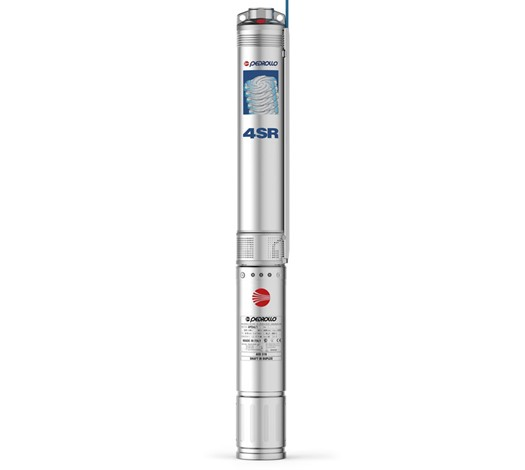
\includegraphics[width=0.35\linewidth]{Pedrollo}
 \captionsetup{justification=centering}
 \caption[Comparable example of the fieldwork submersible pump]{Comparable example of the fieldwork submersible pump \\ (source: \url{https://www.pedrollo.com/en/4sr-4-submersible-pumps/150})} 
 \label{fig:Pedrollo}
\end{figure}

\item Generator \& power converter: Kipor diesel generator - 5 kVA \\
A mobile generator has been used as a pump power source. The Kipor generator is a relatively small model, easy to handle and meets the pump requirements by the use of the 230 V connection. A power converter is placed between generator and pump to manually switch on and off the pump. To facilitate a flawless transfer between generator and pump one should be aware the cables and connections towards the pump should be waterproof. Moreover these power cables should be of a decent length to allow the pump to submerge. 

\begin{figure}[h!]
 \centering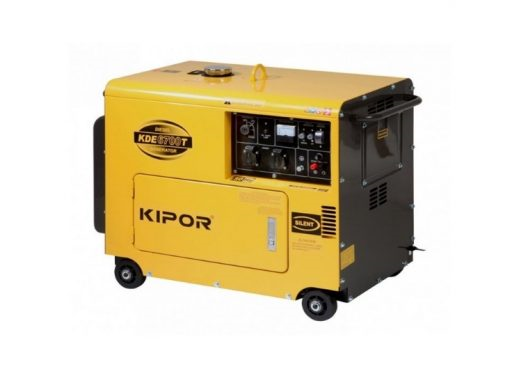
\includegraphics[width=0.40\linewidth]{Kipor}
 \captionsetup{justification=centering}
 \caption[Comparable example of the fieldwork generator]{Comparable example of the fieldwork generator \\ (source: \url{https://www.kipor-power.eu/winkel/kipor-kde6700t-diesel-generator-5-kva/})}
 \label{fig:Kipor}
\end{figure}

\item Hose: \\
As a transport line towards the location of discharge a flexible water hose has been attached to the pump. The hose has been manufactured in Polyethylene, has an external diameter of 1$^{1⁄4}$” and is approximately 100 m long. 

\begin{figure}[h!]
 \centering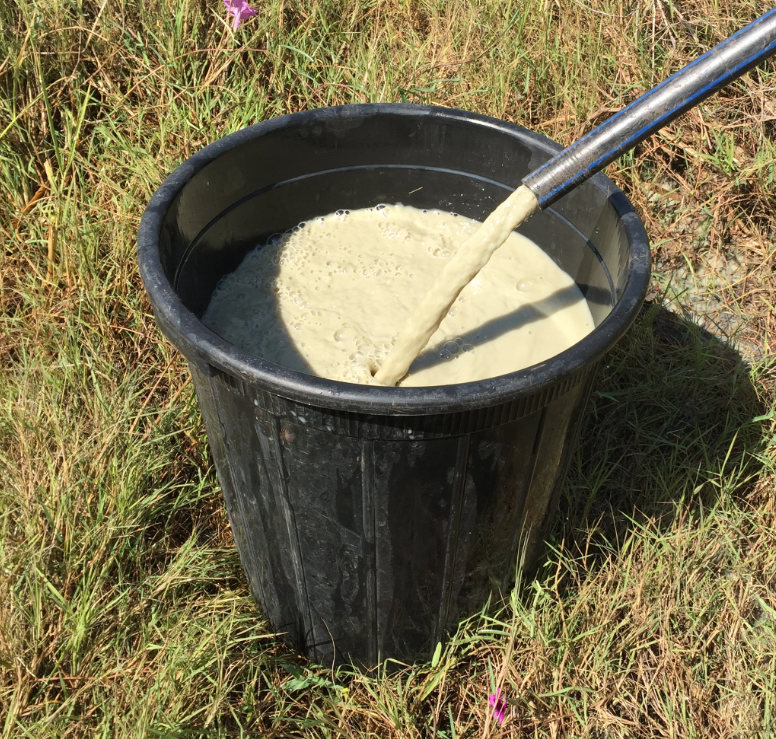
\includegraphics[width=0.35\linewidth]{Hosebucket}
 \captionsetup{justification=centering}
 \caption{Actual fieldwork hose \& bucket}
 \label{fig:Hosebucket}
\end{figure}

\item Bucket: \\
As a rough estimation for discharge an  plastic bucket has been used. This oversized measuring cup stores volumes up to 50 l and contains 5 l level indicators. 

\end{itemize}

\bigskip
\textbf{GWT measurements} 

\begin{itemize}
\item Pressure sensor data loggers: \\
\-- Van Essen; TD-Diver Type DI801 (2x) \& Baro-Diver Type DI800 (1x):\\
TD- and Baro-Divers are applied for the measuring and recording of time dependent fluctuations in (ground)water levels, atmospheric pressures and temperatures. The TD-Divers can record a water column up to 10 m. Baro-Divers can be used to measure atmospheric pressures and shallow water levels, approximately up to a range of 0.9 m. Based on the internal memory these devices can store up to 72.000 measurements per parameter. Measurement logging can be programmed by the use of a USB-Unit and the Diver-Office software. With a battery life of 10 years, long and/or short term measurements can be applied with a sample interval of 0.5 seconds to 99 hours. Moreover the sample interval can be linear or logarithmic.

\begin{figure}[h!]
 \centering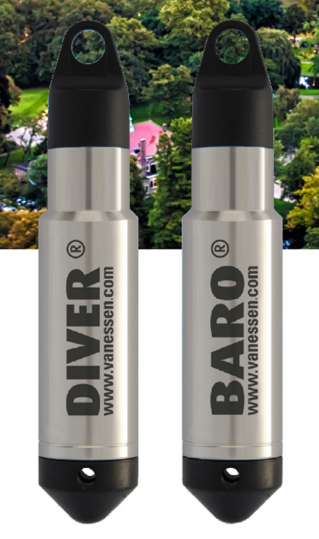
\includegraphics[width=0.17\linewidth]{Essen}
 \captionsetup{justification=centering}
 \caption[Comparable examples of Van Essen TD- \& Baro-Divers]{Comparable examples of Van Essen TD- \& Baro-Divers \\(source: \url{https://www.vanessen.com/images/PDFs/TD-Diver-DI8xx-ProductManual-nl.pdf})}
 \label{fig:Essen}
\end{figure}

\-- In-Situ; RuggedTROLL100 (2x) \& BaroTROLL (1x):\\
Rugged TROLL 100 and BaroTROLL divers are applied for the measuring and recording of time dependent fluctuations in (ground)water levels, atmospheric pressures and temperatures. The RuggedTROLL100 divers function in a pressure range up to 9 m water column. BaroTROLL divers can be used for the measurement of atmospheric pressures, up to 1 bar. The internal memory of 2.0 MB accommodates the storage of 120.000 data records. A record contains a set of three items; date \& time, pressure and temperature. The internal battery has a lifetime of approximately 10 years. By the use of the Rugged TROLL docking-station and the Win-Situ 5 software, linear logging can be programmed. Fastest logging rate is 1 log per second for the Rugged TROLL 100 divers and 1 log per minute for the BaroTROLL divers. Optionally it is possible to display the pressure in units of Psi, Bar, Pascal or mH$_{2}$O. 

%More information on the In-Situ RuggedTROLL100 and BaroTROLL can be found online: \href{https://www.in-situ.com/wp-content/uploads/2014/11/SS\_RuggedTROLL\_100\_200\_Dec2017.pdf}{https://www.in-\\situ.com/wp-content/uploads/2014/11/SS\_RuggedTROLL\_100\_200\_Dec2017.pdf}. (dit laatste tussen de kromme haakjes) is de text die wordt gedisplayed)

\begin{figure}[h!]
 \centering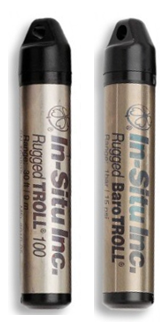
\includegraphics[width=0.17\linewidth]{TROLL}
 \captionsetup{justification=centering}
 \caption[Comparable examples of In-Situ TD- \& Baro-Divers]{Comparable examples of In-Situ TD- \& Baro-Divers \\ (source: \url{https://in-situ.com/product-category/water-level-monitoring/level-temp-data-loggers/})}
 \label{fig:TROLL}
\end{figure}
% hier met \\ een eigen cut-off naar volgende lijn gemaakt, waarbij de ref blijft werken

\item Hand measurement device: Heron water tape \\
The water tape is applied to hand measure static water levels and verify drawdown water levels during the pumping tests. The water tape has a length of 300 ft (100 m). A water level sensing probe is attached to the tail of the tape. Probe water contact results in an instant auditory signal, after which the depth can be determined by eye. Product specifications can be found on the Heron webpage.

\begin{figure}[h!]
 \centering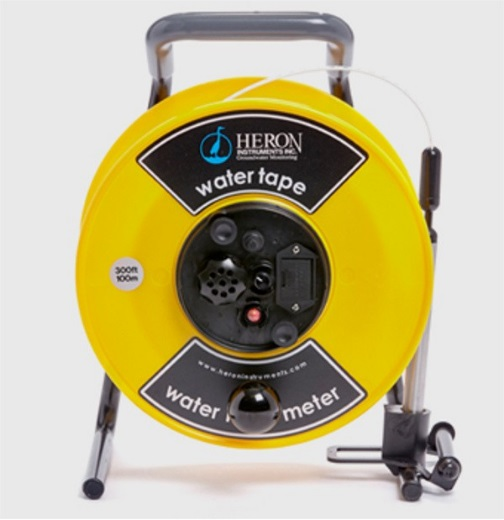
\includegraphics[width=0.35\linewidth]{Heron}
 \captionsetup{justification=centering}
 \caption[Comparable example of the fieldwork water tape]{Comparable example of the fieldwork water tape \\ (source: \url{https://envirotechonline.com/water-level-interface-meters/the-heron-water-tape.html})}
 \label{fig:Heron}
\end{figure}

\end{itemize}

\section{General measurement structure}
\label{section:measurement_structure}
This section accommodates multiple key aspects in the test set-up. By the implementation of this thought-out pumping test and measurement set-up an optimal test result is pursued. Moreover it accommodates information on fieldwork reproduction.
\bigskip \\
\textbf{Pump installation} \\
Based on the log sheets the original (2016) site-specific borehole depths are known in advance. Due to the accumulation of sedimentation the borehole depth decreases over time. To prevent pump damage and make sure properly functioning is maintained, the actual borehole depths are measured before the pumping tests. Outcome of the measurements are taken into account for each individual test set-up. To prevent excessive spread of soil particles the submersible pump is positioned at least 5 meters above the measured bottom. In practice this resulted in a pump suction depth of approximately 35 m for every individual pumping test.
\bigskip \\
\textbf{Discharge (measurement)} \\
A single 100 m hose is directly connected to the outlet of the submersible pump. Based on the pump position (deep inside borehole), a length of circa 60 m is still present for the horizontal displacement of water. At this distance (relative to the borehole) water is discharged on the surface.
\\
The head of the hose is equipped with a nozzle to roughly regulate the dis-charge rate. By the use of this nozzle, discharge rates in the range of 50-75 m$^{3}$/d are obtained during the pumping tests. Rates are measured by the use of a 50 l bucket. Starting at the moment of pump operation, the duration of filling is measured twice every 15 minutes. The average is used to calculate the time dependent discharge rates. More detailed discharge information can be found in the site-specific fact-sheets below.
\bigskip \\
\textbf{GWT measurement} \\
Drawdowns due to pumping tests are preferably measured in multiple piezometers located at a certain known horizontal distance from the discharge well \citep{Kruseman2000}. In the northern Ghana surroundings, close range monitoring options are absent. Due to a lack of time and/or resources these facilities cannot be arranged either. Moreover, the implementation of such facilities do not match research nature. Aim of this research is to collect fieldwork data by the use of minimal resources. The local absence of abundant measurement options strengthens this approach. In this research pumping test GWT drawdowns are measured in the discharge well only.\\
A water tape (hand equipment) is used, first of all to determine the initial (static) GWT. Subsequently the device is applied as a real time indicator of drawdown. During the pumping test multiple hand measurements are applied at randomly picked moments to monitor test progress. Gathered data functions as verification and back-up of the pressure sensors, which are normative.
\bigskip \\
Two types of divers (different brands) are used as basic GWT measurement devices. Specifications show these divers can respectively measure pressures up to 10 m (Van Essen) and 9 m (In-Situ) water column (bron..). The northern Ghana regional subsurface is characterized as highly heterogeneous. The pumping test GWT drawdown order of magnitude is therefore unpredictable. To prevent the occurrence of missing drawdown data, the single borehole accommodates multiple divers at ascending depths. The water column between the initial static water table and pump position is preferably filled with about four divers, with a mutual distance that meets the divers range specifications. To make sure the divers stay in position they are leashed to a rope which runs from well top to pump. This measurement set-up forms a robust network for the collection of drawdown data. \\
Practical circumstance can however cause the application of a more simplified set-up. One can think of a situation in which the pump is already installed and/or will not be removed at the end of the pumping test. Rope attachment of the divers to the pump is in this case no longer possible. Adverse effect of the simplified set-up is a data collection which is more vulnerable. To prevent the occurrence of undesired diver movement a minimum distance of 5-10 m between pump and lowest diver is implemented in the simplified set-up. A complete overview of the borehole measurement set-up (desired and simplified) can be found in figure~\ref{fig:set-up}. \\

\begin{figure}[h]
	\centering
	\begin{subfigure}[b]{0.4\linewidth}
		\centering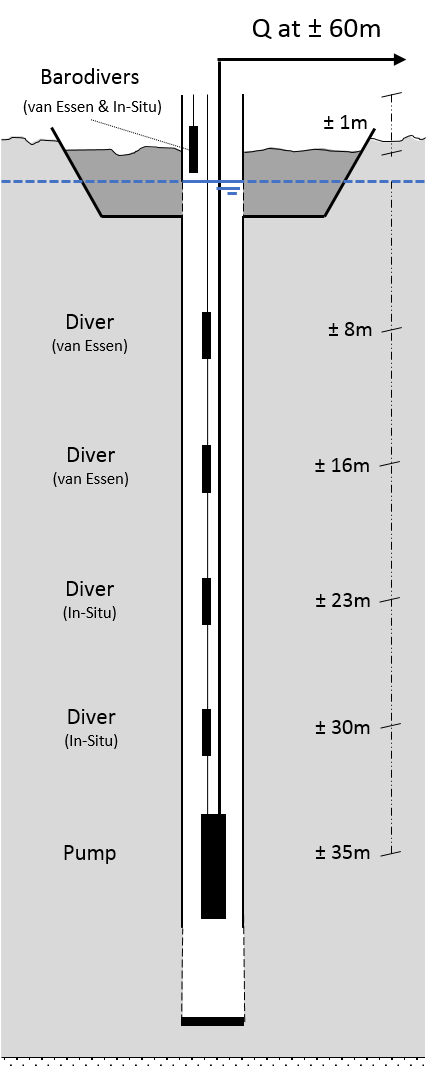
\includegraphics[width=0.75\linewidth]						{Setup_pumping_test.png}
		\captionsetup{justification=centering}		
		\caption{\label{fig:general}}
		\end{subfigure}%\hfill
	\begin{subfigure}[b]{0.4\linewidth}
        \centering\includegraphics[width=0.75\linewidth]						{Setup_pumping_test_bingo.png}
		\captionsetup{justification=centering}		
		\caption{\label{fig:simplified}}
		\end{subfigure}
	\captionsetup{justification=centering}	
	\caption{Fieldwork (measurement) set-up (\subref{fig:general}) general, ~(\subref{fig:simplified}) simplified} 
	\label{fig:set-up}
\end{figure} 

Besides the divers the measurement set-up also accommodates two Baro-divers (van Essen \& In-Situ), positioned in the borehole top section. Drawdown is by definition expressed as time dependent GWT reductions relative to the initial status. Short term atmospheric fluctuations in pressure are compared to the water pressures negligible small. Nonetheless these minor atmospheric influences are also included in the data collection. The inclusion of these Baro-diver measurements increases measurement accuracy, especially with respect to the multi-day system monitoring.
\bigskip \\
The exact start of pump operation could not be determined in advance. To avoid unnecessary risks in missing out on the collection of drawdown data, all pressure sensors are programmed to start logging well in time (08:00:00, local time, at pumping test days). All divers are set to log with a similar linear interval of 10 seconds. Only exception is the In-Situ BaroTROLL, which is programmed to linear log at its minimum sample interval; once a minute. 


\section{Site-specific measurement results}
\label{section:fieldworkresults}
In consultation with Conservation Alliance (CA), a total of five pumping tests are applied in boreholes located at Bingo, Nungo, Nyong Nayili and Janga. By the use of a fifth borehole, location Ziong, the day-to-day PIT system-use is monitored for a week. All tests are applied in November-December 2017, shortly after the transition from wet to dry season. Geohydrological data is gathered by the application of the general pumping test set-up (as described above) at the location Nungo, Nyong Nayili and Janga. The simplified set-up is applied at the location Bingo and Ziong. Outcome of the tests are widespread. Detailed site-specific results are displayed in the fact-sheet figures below (Figures ~\ref{fig:Bingo} -~\ref{fig:Ziong}).

\begin{figure}[h!]
 \centering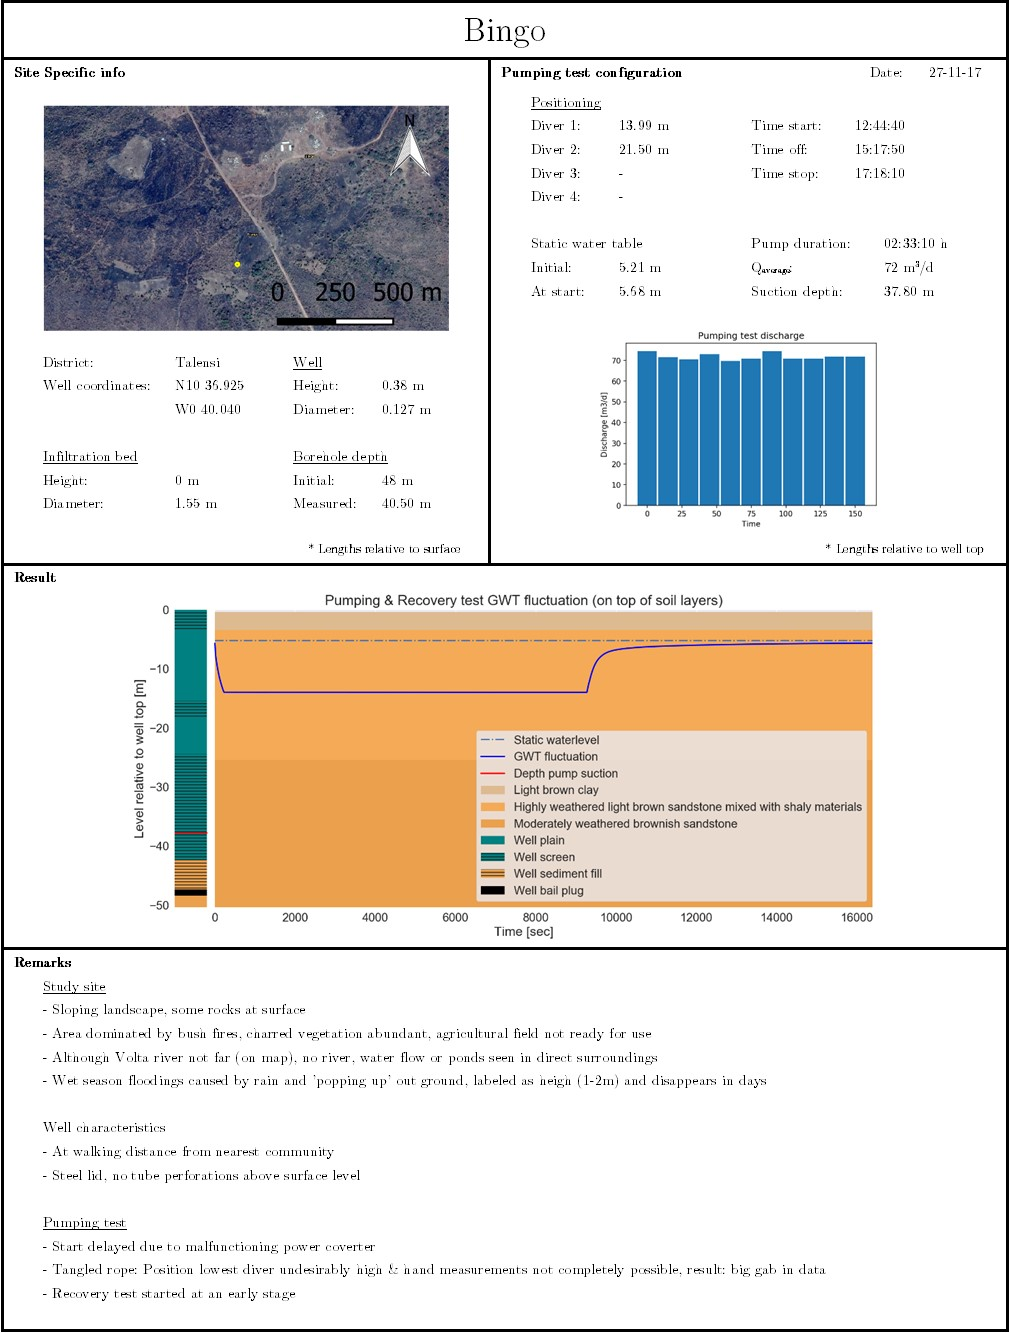
\includegraphics[width=\linewidth]{Bingo.jpg}
 \captionsetup{justification=centering}
 \caption{Fieldwork fact-sheet: Bingo}
 \label{fig:Bingo}
\end{figure} 

\begin{figure}[h!]
 \centering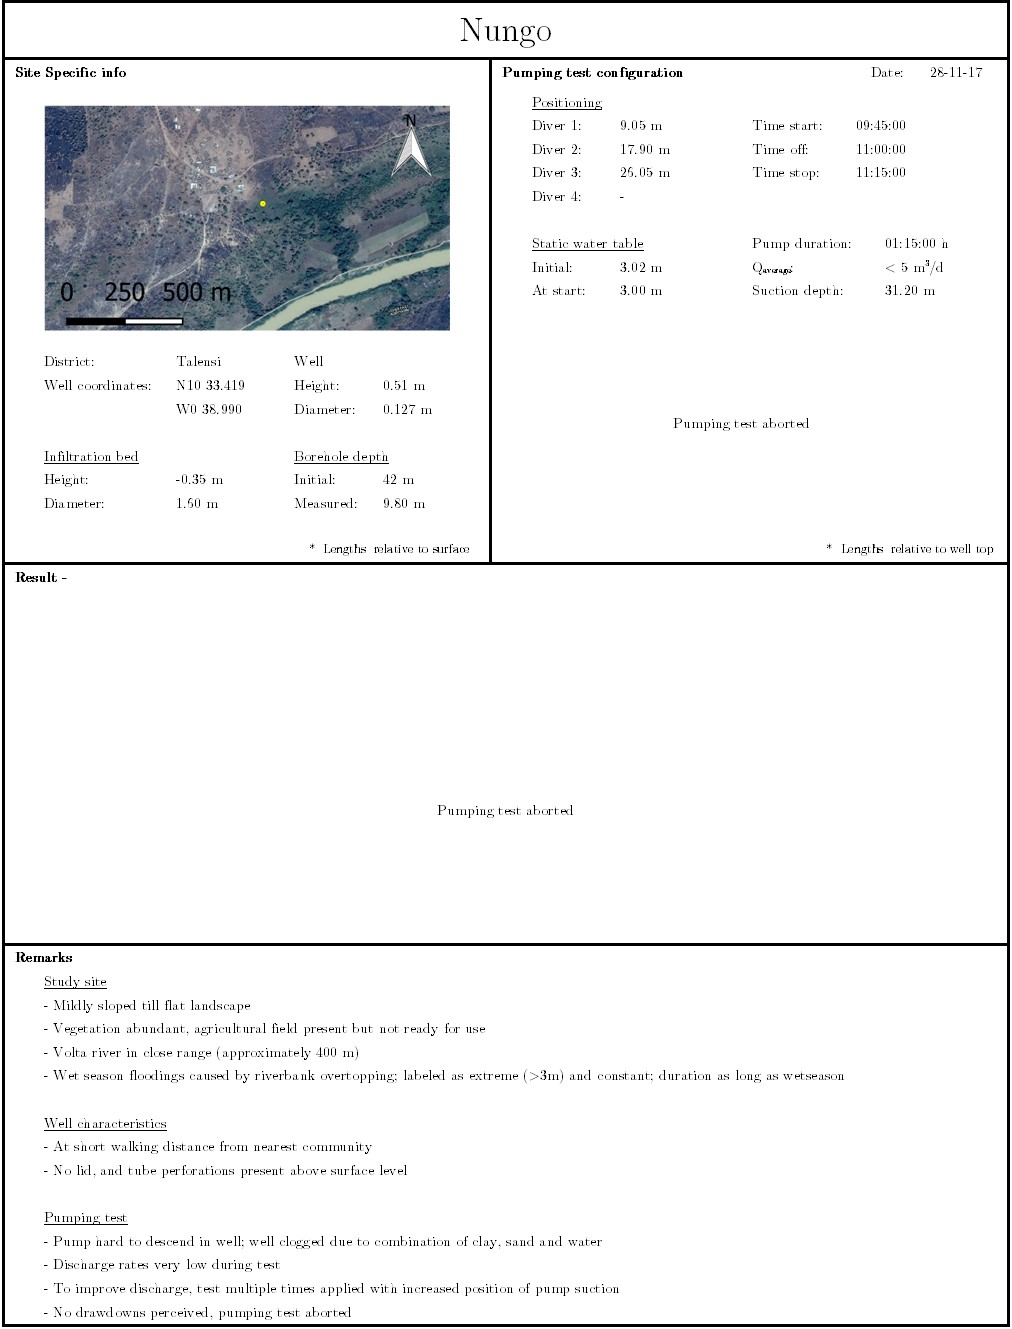
\includegraphics[width=\linewidth]{Nungo.jpg}
 \captionsetup{justification=centering}
 \caption{Fieldwork fact-sheet: Nungo}
 \label{fig:Nungo}
\end{figure} 

\begin{figure}[h!]
 \centering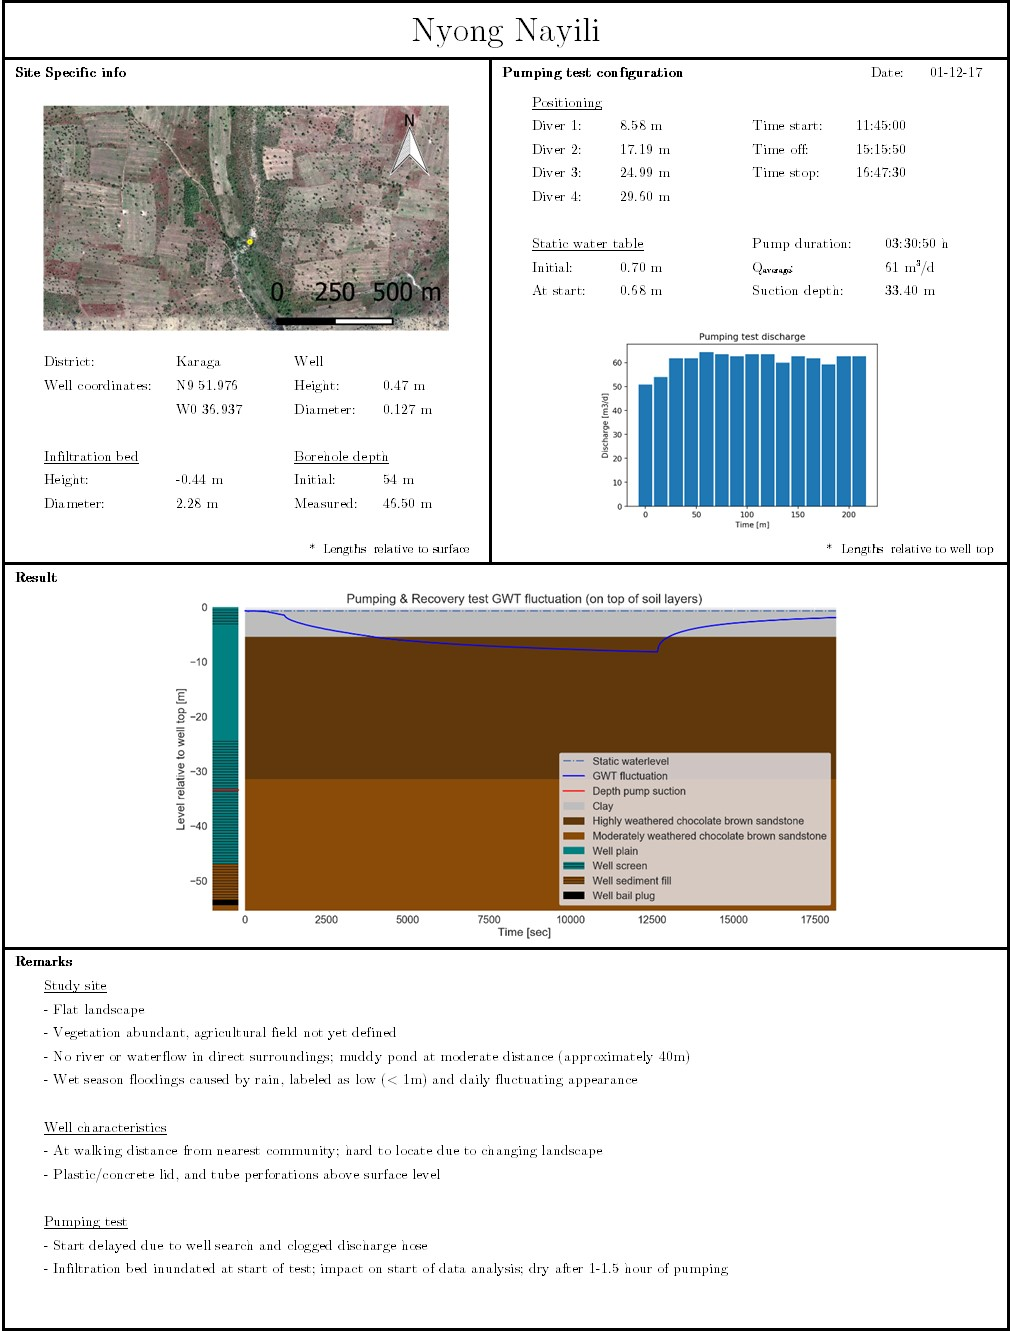
\includegraphics[width=\linewidth]{Nyong_Nayili.jpg}
 \captionsetup{justification=centering}
 \caption{Fieldwork fact-sheet: Nyong Nayili}
 \label{fig:Nyong_Nayili}
\end{figure} 

\begin{figure}[h!]
 \centering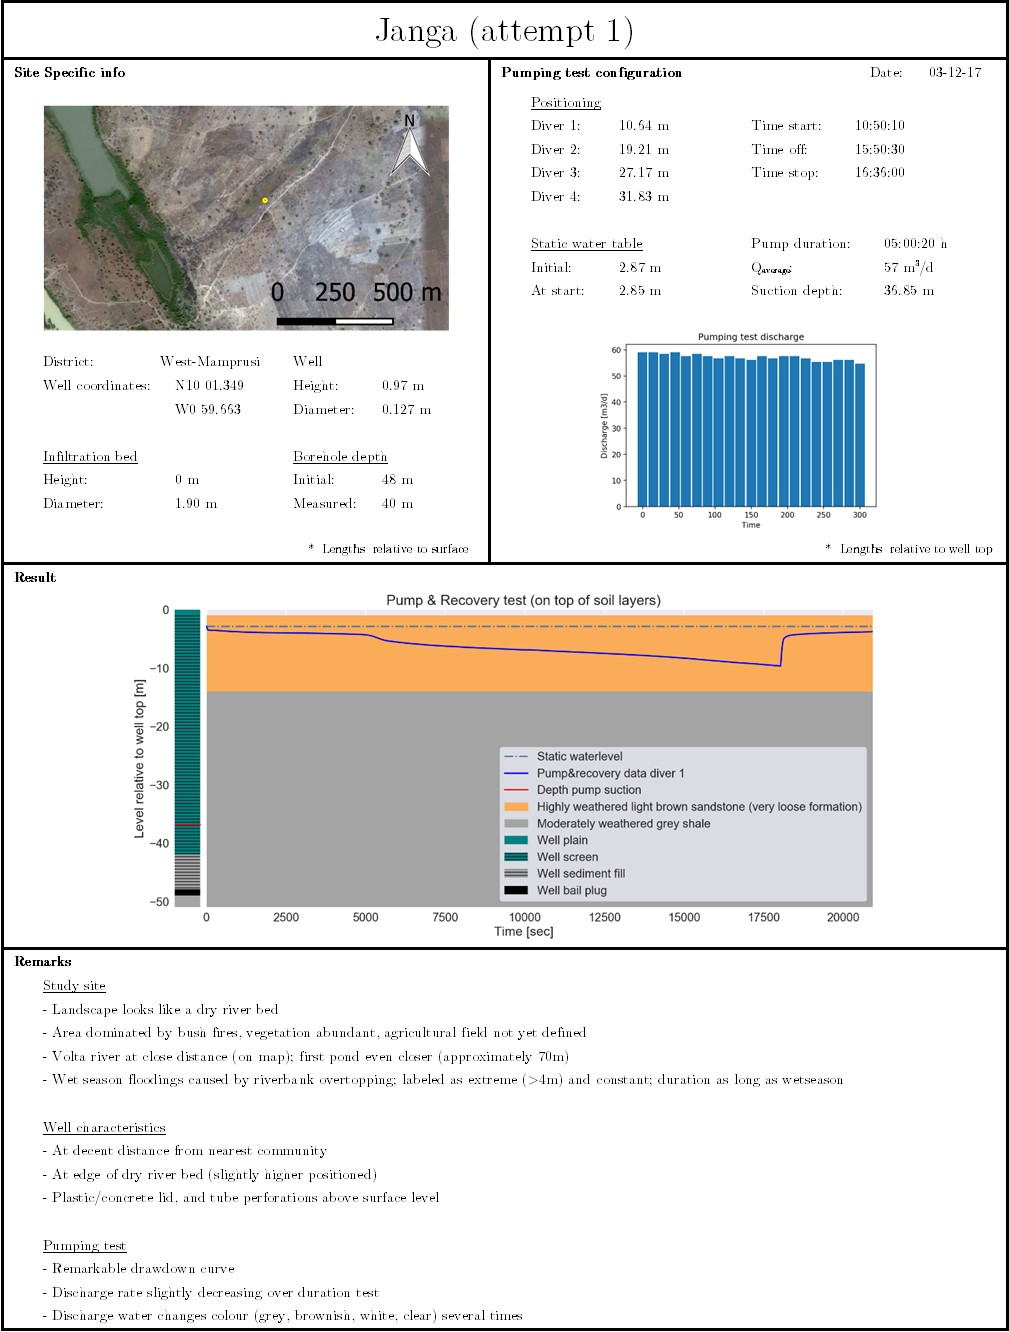
\includegraphics[width=\linewidth]{Janga1.jpg}
 \captionsetup{justification=centering}
 \caption{Fieldwork fact-sheet: Janga (attempt 1)}
 \label{fig:Janga1}
\end{figure} 

\begin{figure}[h!]
 \centering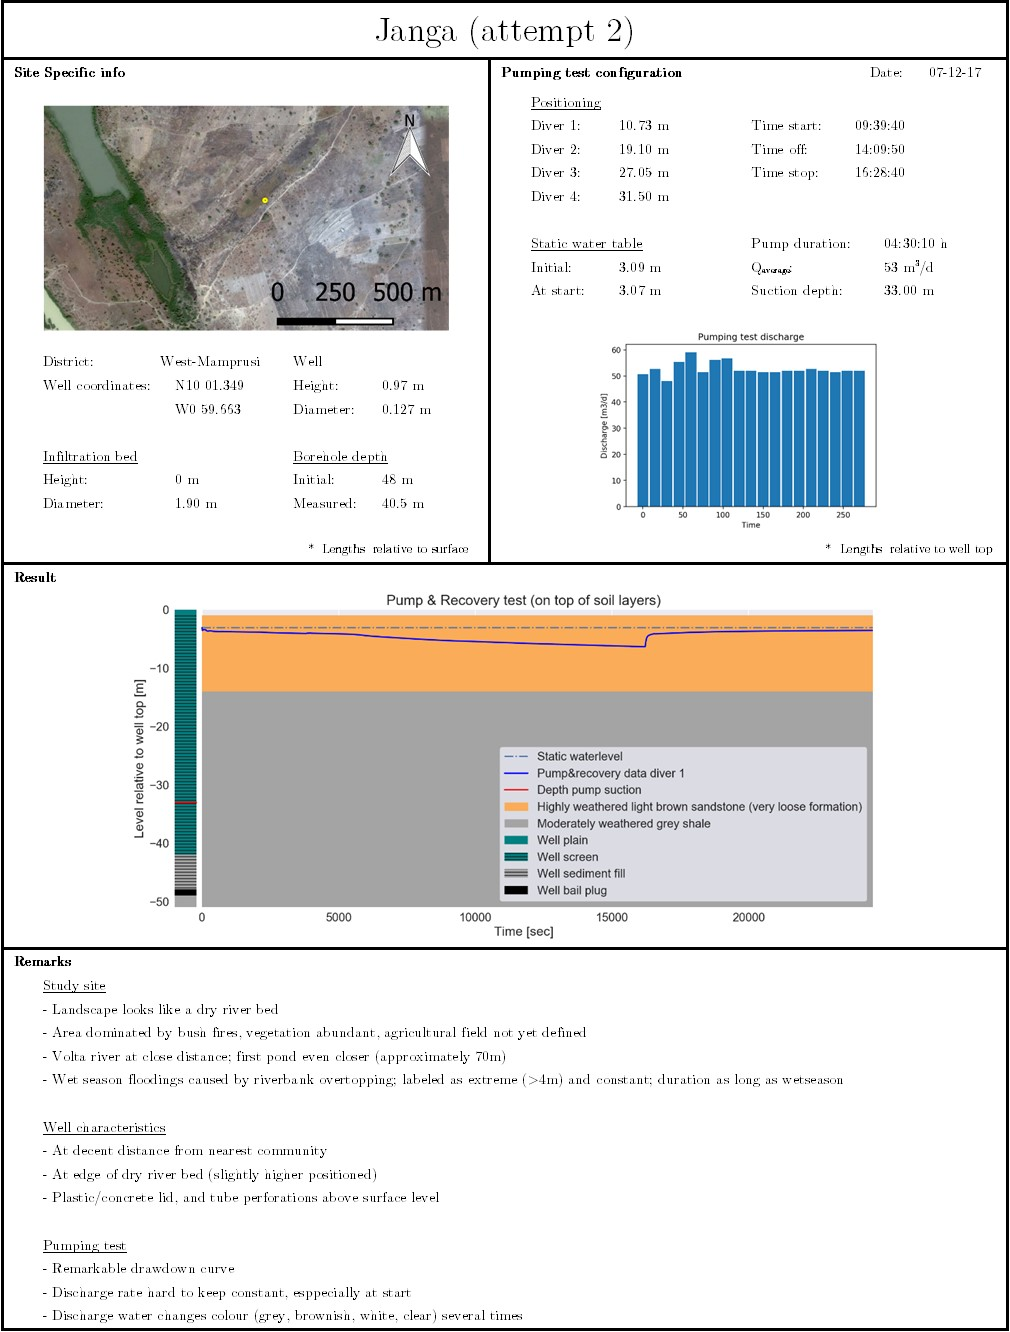
\includegraphics[width=\linewidth]{Janga2.jpg}
 \captionsetup{justification=centering}
 \caption{Fieldwork fact-sheet: Jamga (attempt 2)}
 \label{fig:Janga2}
\end{figure} 

\begin{figure}[h!]
 \centering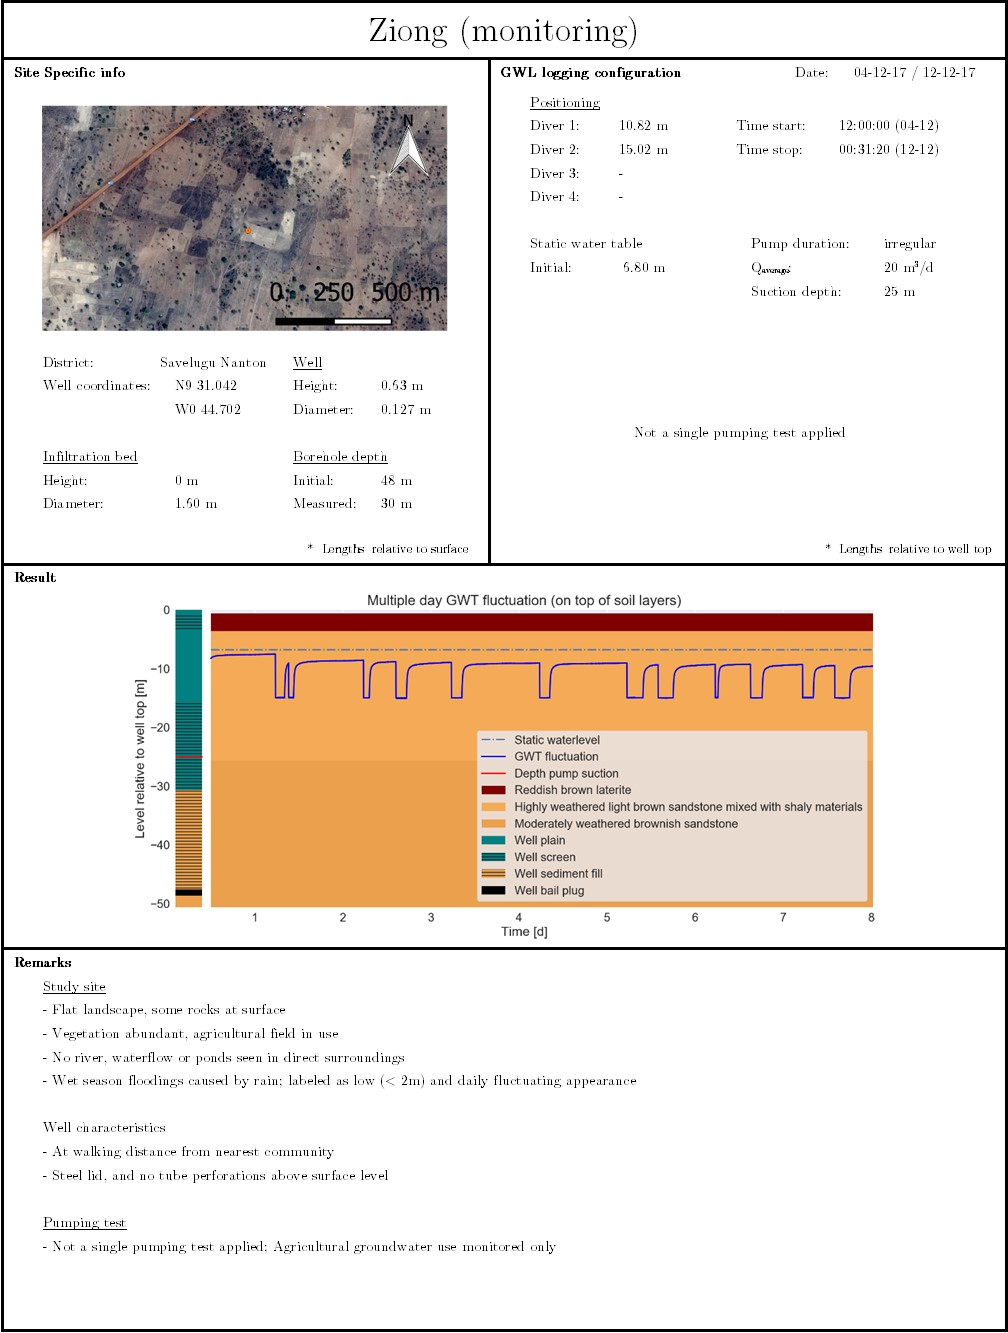
\includegraphics[width=\linewidth]{Ziong.jpg}
 \captionsetup{justification=centering}
 \caption{Fieldwork fact-sheet: Ziong (location of monitoring)}
 \label{fig:Ziong}
\end{figure} 